\section{Evaluation}\label{ch:evaluation}

\subsection{Evaluation Framework}
In order to make the evaluation of our agent easier and less time-consuming, we build an evaluation framework capable of automated running agents and analysis of the performance. Doing that, it is possible to compare the performance of our agent at the current state of development with the other teams' agents made publicly available on the aibirds forum. Having the possibility to easily evaluate the agent helps to detect problems with specific levels, but more important, it shows whether changes made to the code affect the performance of the agent on levels where it was not expected. \\
The evaluation framework consists of three parts, each of it wrapped into an own class: The class main defines the command line user interface, which can be used to choose the levels and agents. The class automatically copies the desired levels into the level folder of the game, such that those levels are loaded when the game is started. There are all levels of the previous competitions available. Also, it is possible to load levels generated by yourself (this can be done by using the level generator). \\
The class logger is responsible for starting the game, starting the agents on the desired levels and logging the achieved scores. The logging is implemented by filtering the console output of ABServer. The results are stored into an csv-file. The class logs continuously, so it is possible to have a look at the performance while the test is still running.\\
Finally, the class evaluator offers an command line user interface and the logic for analyzing the logged scores of the agents and generating bar charts which show the performance of the agents. As a result, a pdf file is created which holds 3 kinds of bar charts for every level: First, a chart which shows the mean score of an agent, e.g., the average score of an agent over all runs of the level. The second chart shows the median of the scores. The last type shows the highest score (max-score) an agent has achieved on the specific level. This one is the most important chart, because if the evaluation is conducted under competition conditions, the highest score is the only one that counts. Additionally, there is a chart at the end of the pdf which shows the sums of all highest scores. This is also the measurement used in the finals of the competition.\\
The evaluation framework was entirely written in python. This allowed us to write compact, easy-to-read code. Python also allows an uncomplicated access to data analysis tools and, as a scripting language, is more suitable for pipeline-like architectures than Java. \\
Examples of the charts generated by evaluator.py can be found in figure \ref{fig:output1} and \ref{fig:output2}

\begin{figure}%[t] 
	\centering 
	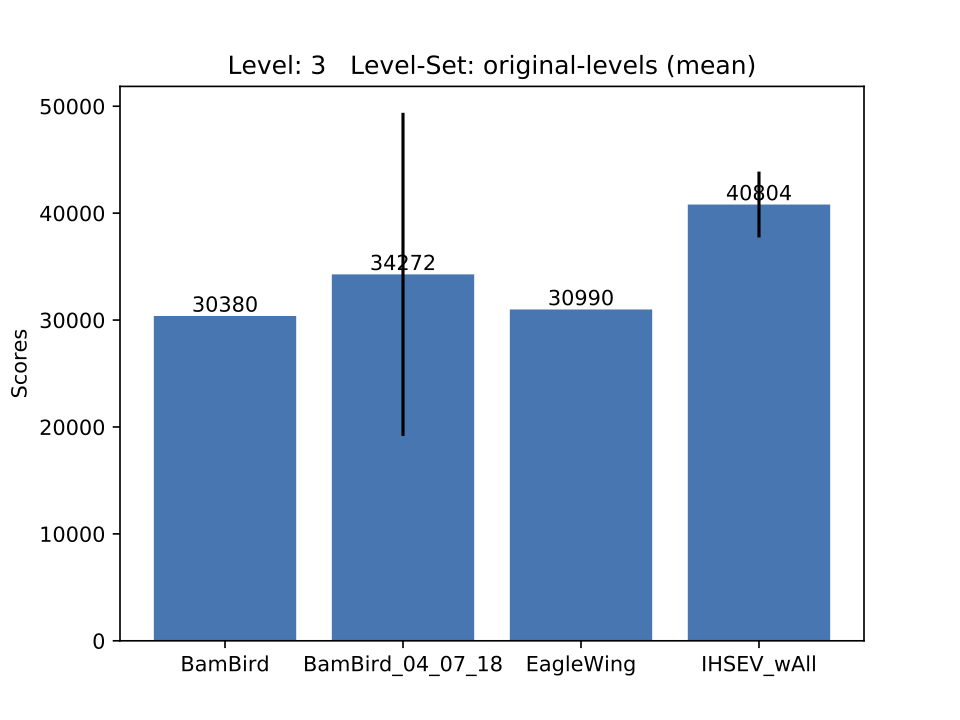
\includegraphics[width=50mm]{img/evaluation_results_05_07_18_11_20_33_original_levels.png}
	\caption{The evaluation of a preliminary BamBird 2018 agent against other teams' agents on the third level of the original levels (Poached Eggs). The bar chart shows the agents' average score on the level.\label{fig:output1}}
\end{figure}

\begin{figure}%[t] 
	\centering 
	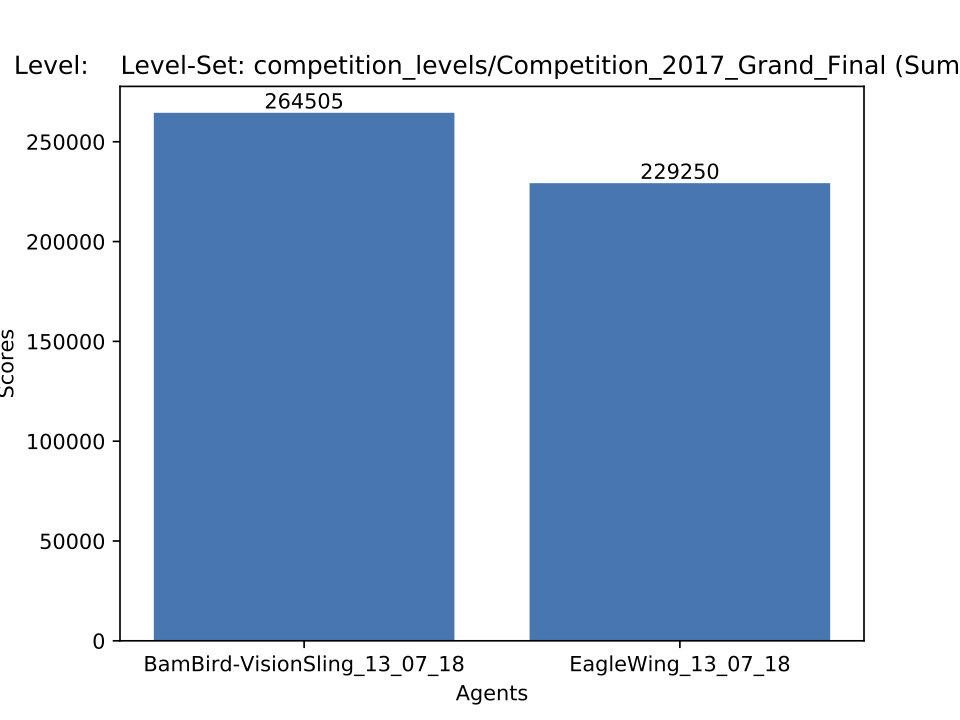
\includegraphics[width=50mm]{img/evaluation_results_13_07_18_21_17_06_grand_final_2017.png}
	\caption{The evaluation of the final BamBird agent against EagleWing 2017 on the grand final of 2017. The chart shows the sum of the highest score of every on all 8 levels.\label{fig:output2}}
\end{figure}

\subsection{Evaluation results}
In order to evaluate the final agent, we performed a benchmark which consisted of a 60 minutes run on the first stage of the Poached Eggs levels. While the agent of 2017 scored 663940 points in this benchmark (see project report 2017), the 2018 agent was able to score 871050 points, which shows that the changes of 2018 improved the agent. The results of the benchmark are presented in table \ref{tab:stage1}.
\begin{table}[h]
	\begin{center}
		\begin{tabular}{l | r r r r}
			Level       & First try & Second try & Third try & Max. points \\
			\hline
			\hline
			Level 1-1   &  30080 &  29750  & 30870   &   30870 \\
			\hline
			Level  1-2  &  53530 &  53480  &  53480  &   53530 \\
			\hline
			Level  1-3  &  30800 &  30760  & 30800   &   30800 \\
			\hline
			Level  1-4  &  28540 &  28360  & 28480   &   28540 \\
			\hline
			Level  1-5  &  57230 &  53270  &  55770  &   57230  \\
			\hline
			Level  1-6  &  15800 &  17140  &   17110 &   17140 \\
			\hline
			Level  1-7  &  25350 &         &         &   25350 \\
			\hline
			Level  1-8  &  57320 &  57080  &  56900  &   57320 \\
			\hline
			Level  1-9  &  0     &  20840  &         &   20840 \\
			\hline
			Level  1-10 &  0     &  54940  &         &   54940      \\
			\hline
			Level  1-11 &  49570 &  49450  & 48490   &   49570      \\
			\hline
			Level  1-12 &  47870 &  55300  &  54770  &   55300 \\
			\hline
			Level  1-13 &  26200 &  35030  &         &   35030      \\
			\hline
			Level  1-14 &  47100 &  62970  &  62970  &   62970 \\
			\hline
			Level  1-15 &  48170 &  48160  &   48170 &   48170      \\
			\hline
			Level  1-16 &  61070 &  62330  &  64310  &   64310 \\
			\hline
			Level  1-17 &  44660 &  45820  &         &   45820 \\
			\hline
			Level  1-18 &  0     &  43020  &  39920  &   43020 \\
			\hline
			Level  1-19 &  37820 &  30390  &  30360  &   37820 \\
			\hline
			Level  1-20 &  44700 &  52480  &         &   52480 \\
			\hline
			Level 1-21  &  0     &         &         &   0 \\
			\hline
			\hline
			SUM         &  &  &   &  871050
		\end{tabular}
	\end{center}
	\caption{Results of the benchmark for the first stage of Poached Eggs\label{tab:stage1}}
\end{table}
